\documentclass{standalone}

\usepackage{color}
\usepackage{tikz}
\usetikzlibrary{positioning}


\definecolor{myred}{RGB}{175,53,71}
% \definecolor{myred}{RGB}{255,127,0}
\definecolor{myblue}{RGB}{0,116,188}

\tikzset{
		edgeStyle/.style = 	{line width = 1.3pt},
		fixed/.style = 		{line width = 1.2pt, color=myred, text=black, circle, draw},
		free/.style=	{circle,draw,minimum size=20},
		node distance=2.3cm
}

\begin{document}
	
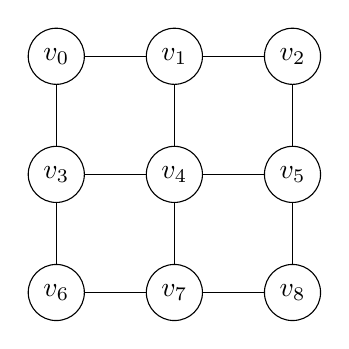
\begin{tikzpicture}
  \foreach \x in {0,...,2}
    \foreach \y in {0,...,2} 
       {\pgfmathtruncatemacro{\label}{\x - 3 *  \y + 7 - 1}
       \node [free]  (\x\y) at (1.5*\x,1.5*\y) {$v_\label$};} 

  \foreach \x in {0,...,2}
    \foreach \y [count=\yi] in {0,...,1}  
      \draw (\x\y)--(\x\yi) (\y\x)--(\yi\x) ;

\end{tikzpicture}	

\end{document}
